\section*{Data}
The first data-set employed is web-scraped Aldermanic voting data. This data set contains 123 observations of determining election outcomes. 
Determining election indicates that an election determined who got the office. 
We remove elections where the general election outcome became a runoff to avoid double-counting. 
For the discrete-choice modeling, we use a reduced form of the Aldermanic voting data, with only observations from 2015 and 2019, so we have data on off-menu expenditures from the year before the election. 
Secondly, there are Aldermanic menu expenditures, which contain the yearly allotted allocations from Aldermen and their respective locations from 2012 to 2020. 
This data set contains 450 ward-year observations of the amount of money spent on off-menu items and on-menu items. 
For the DiD analysis, we will use the entire 450 observation data set, but for the regression discontinuity study, we will use only the 123 observations that correspond to the year after an election. 
This data-set comes from the Office of Budget and Management of the city of Chicago \cite{MenuProgramChoices}. 

The data set employed for the regression discontinuity analysis consists of 123 electoral observations across three elections. 
We can see a large standard deviation of off-menu expenditures consisting of approximately 10\% of the budget each alder-person is allocated. 
Furthermore, we can see that, on average, we expect the electoral outcomes of these contests to be heavily skewed towards the incumbent, with an average incumbent vote share of 65.5\%. The summary statistics for the regression discontinuity is below:


% Table created by stargazer v.5.2.3 by Marek Hlavac, Social Policy Institute. E-mail: marek.hlavac at gmail.com
% Date and time: Tue, Jan 24, 2023 - 08:34:01 PM
\begin{table}[!htbp] \centering 
  \caption{} 
  \label{} 
\begin{tabular}{@{\extracolsep{5pt}}lccccc} 
\\[-1.8ex]\hline 
\hline \\[-1.8ex] 
Statistic & \multicolumn{1}{c}{N} & \multicolumn{1}{c}{Mean} & \multicolumn{1}{c}{St. Dev.} & \multicolumn{1}{c}{Min} & \multicolumn{1}{c}{Max} \\ 
\hline \\[-1.8ex] 
off\_menu & 105 & 49,364.090 & 118,693.100 & 0.000 & 705,155.000 \\ 
votepct & 105 & 59.639 & 11.130 & 32.262 & 86.038 \\ 
\hline \\[-1.8ex] 
\end{tabular} 
\end{table} 


The histogram of off-menu expenditures data employed in the regression discontinuity is below. 
In this, we see that the vast majority of wards spend \$0 on off-menu items, but a small minority of alderpersons seem to use off-menu expenditures. 
We also see that the right tail of the distribution is quite long, so not only are off-menu expenditures rare, but the ward may be spending a large amount of money when they happen.

\begin{figure}[H]
    \centering
    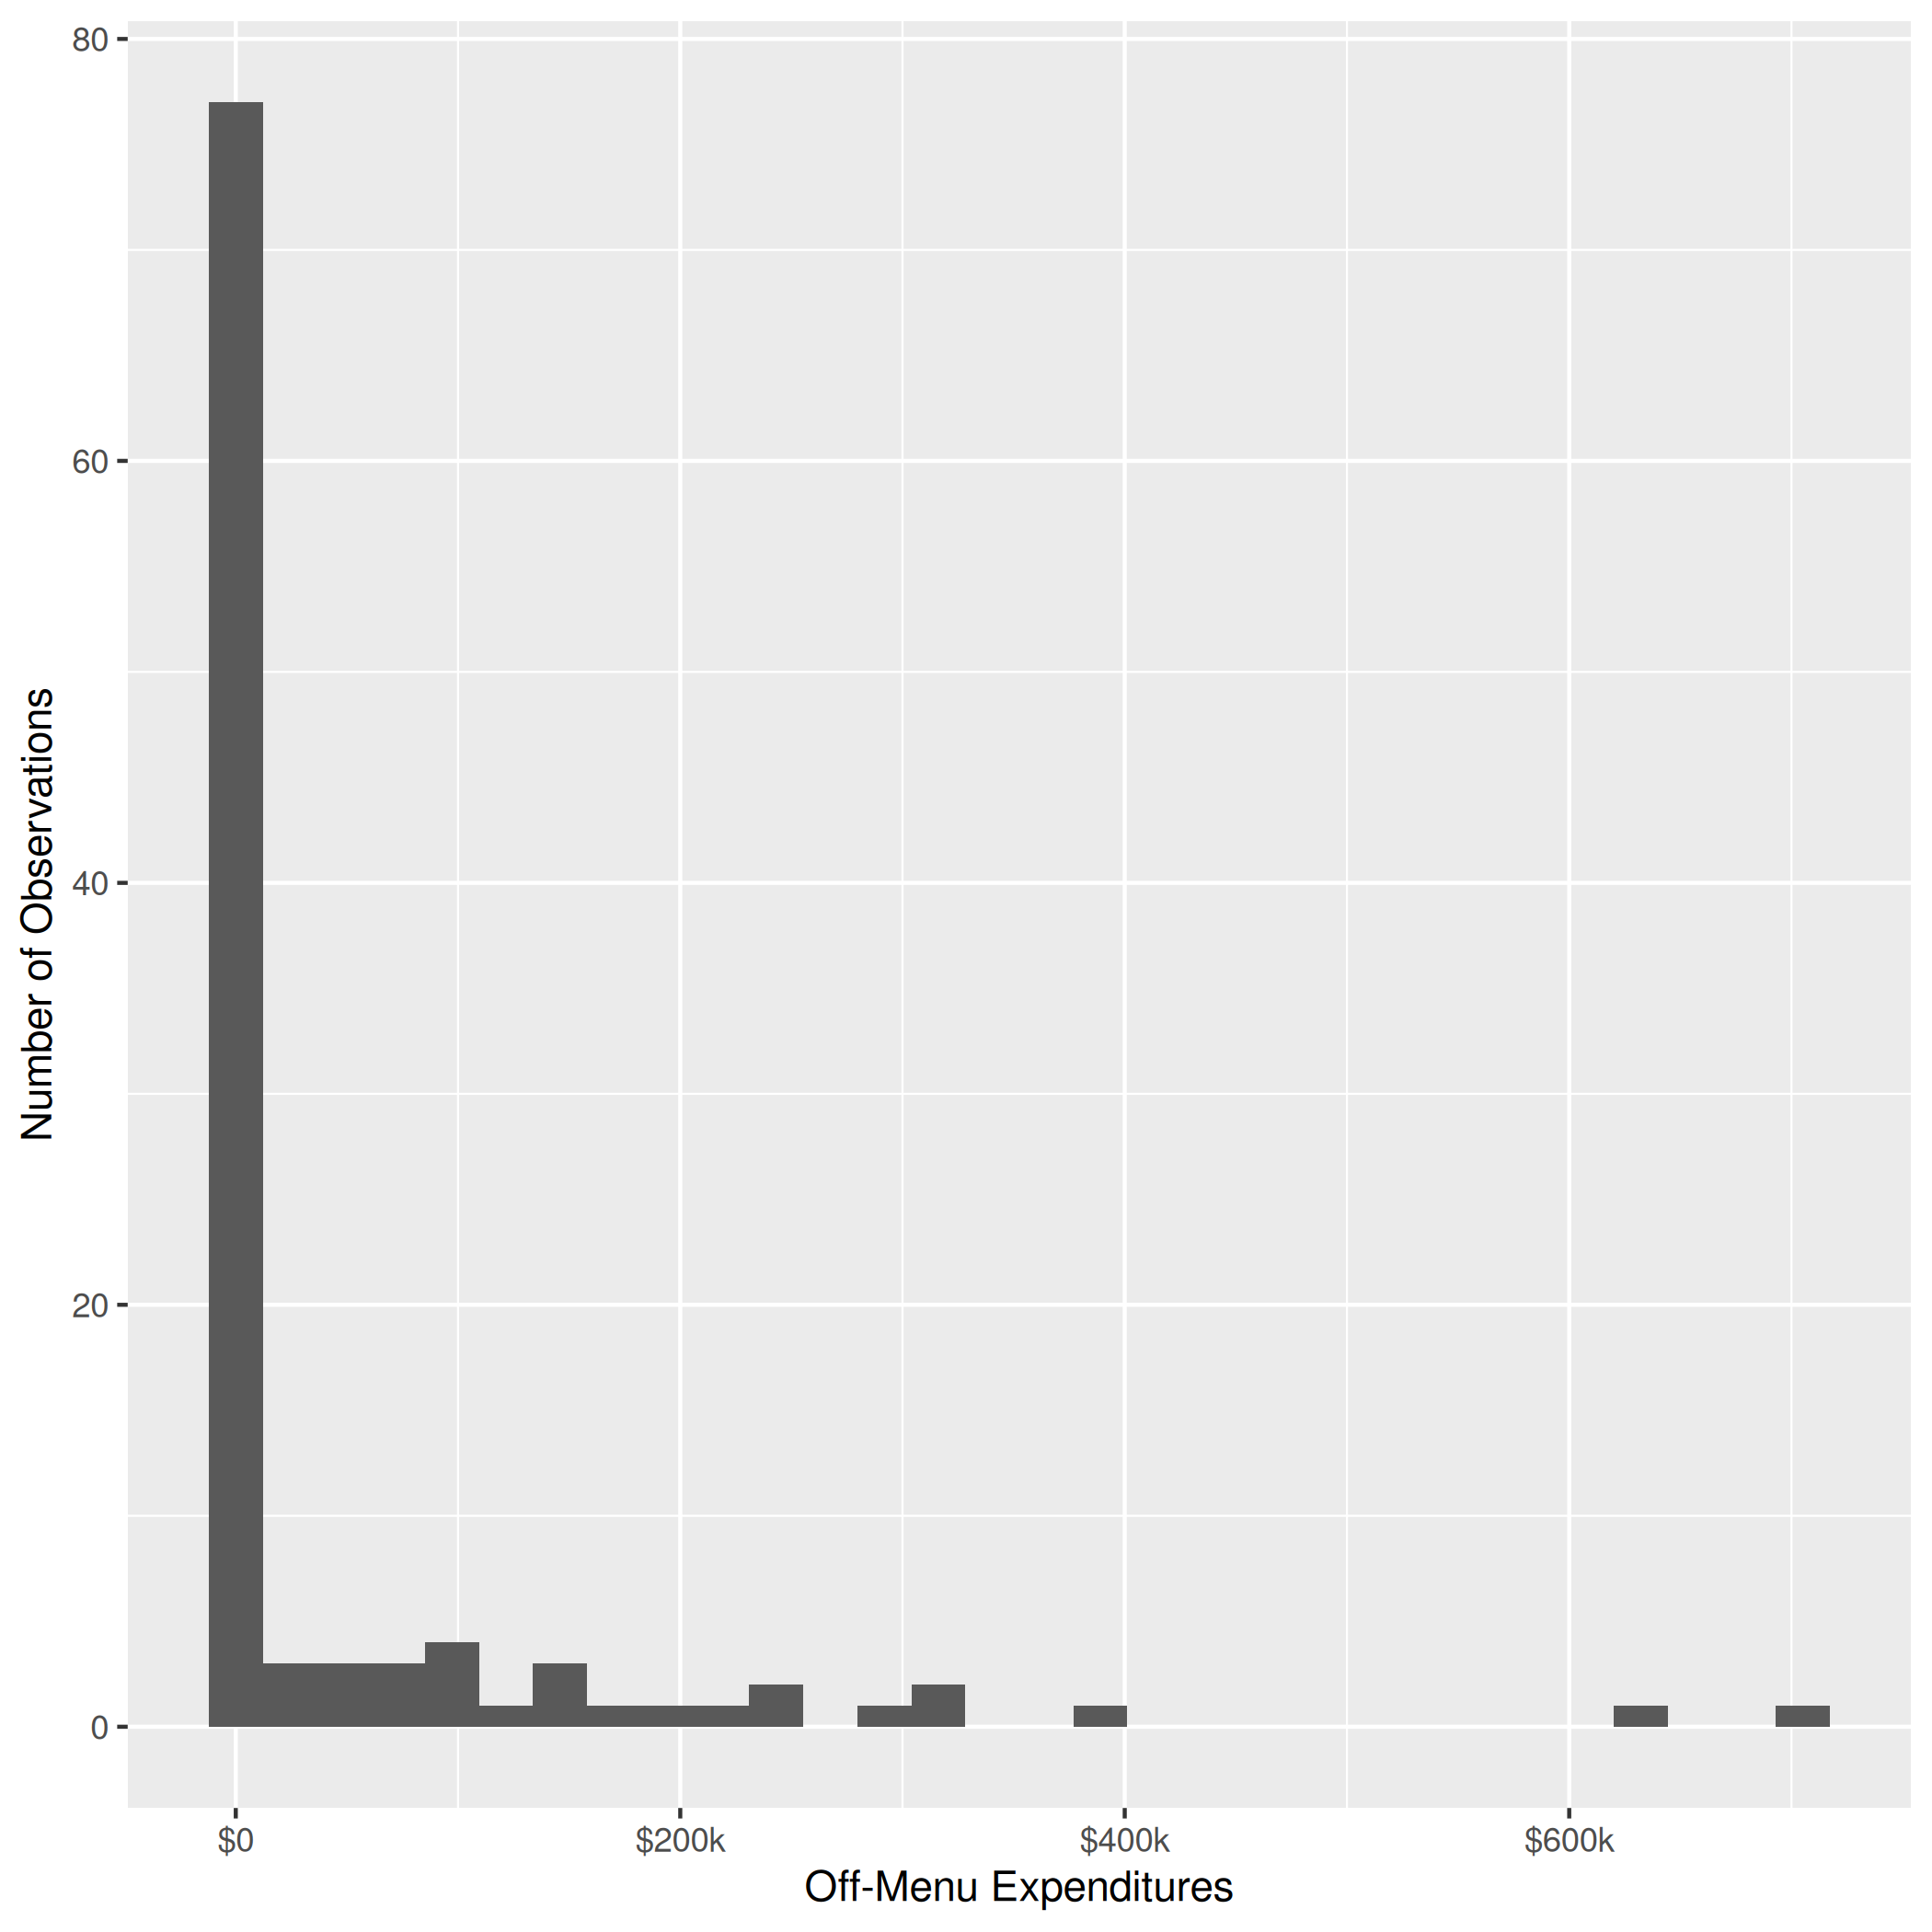
\includegraphics[scale=1]{input/off_menu_expenditures_histogram.png}
    \caption{Histogram of Off-Menu expenditures in 2012, 2016, and 2020 for the RD Analysis}
    \label{fig:my_label}
\end{figure}

A histogram of incumbent vote-shares used in the regression discontinuity analysis is shown below. 
Here we see that the distribution is quite irregular, featuring what seems to be a large discontinuity at the cutoff of 50\% with large density discontinuities elsewhere. 
The histogram shows that the data does not easily fit into a, say, a normal or some other kind of distribution. 
This is likely a reflection of the low number of observations.  

\begin{figure}[H]
    \centering
    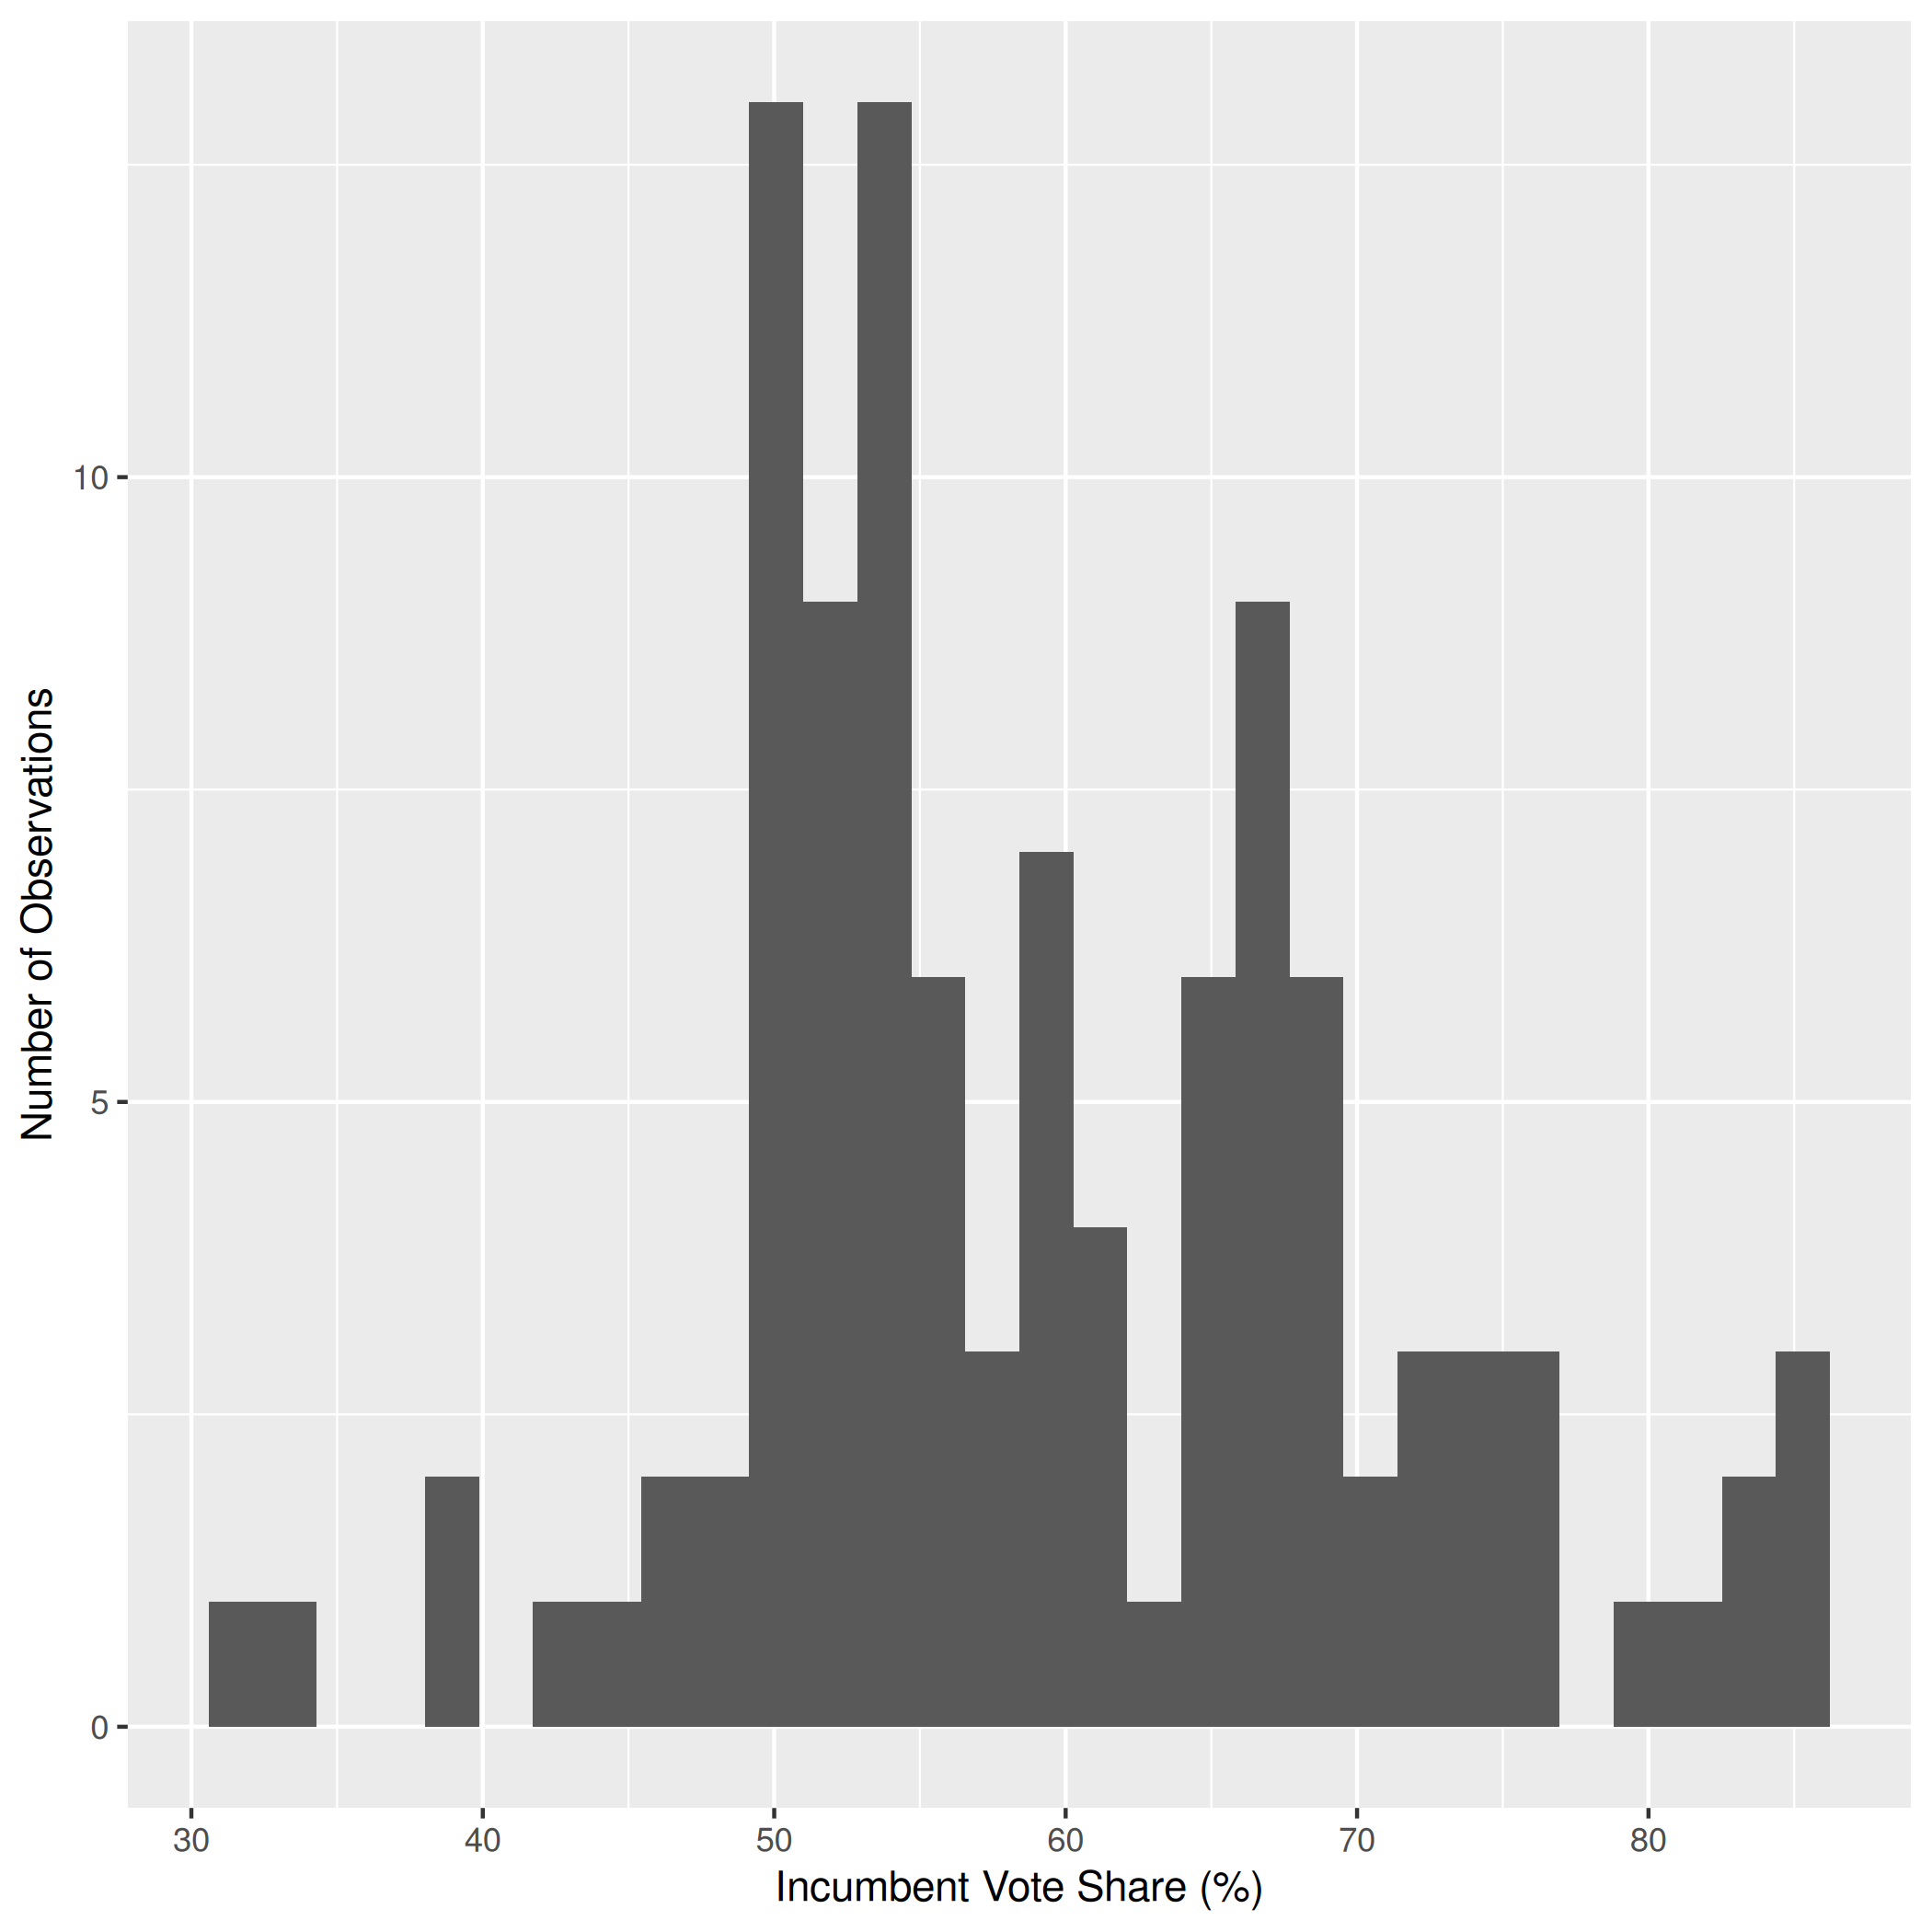
\includegraphics[scale=1]{input/voteshare_histogram.png}
    \caption{Histogram of Incumbent Voteshares in 2011, 2015, and 2019 for the RD analysis}
    \label{fig:my_label}
\end{figure}

The Differences-in-differences data set comprises 450 observations of off-menu expenditures across 50 wards over nine years from 2012-2020. 
Twelve wards are ``treated'' with a leaving incumbent, of which six lost the election, and six retired \cite{election_results}. 
From the summary statistics of the data below, we can see that the treatment group makes up approximately a quarter of the data set and that average off-menu expenditures are lower in the group of wards that had an alderman retire or defeated in a reelection attempt. 

\begin{table}[H] \centering 
  \caption{Summary Statistics for Diff-in-Diff Analysis} 
  \label{} 
\begin{tabular}{@{\extracolsep{5pt}} cccccc} 
\\[-1.8ex]\hline 
\hline \\[-1.8ex] 
 Treatment Group & N & Mean & St. Dev & Min & Max \\ 
\hline \\[-1.8ex] 
treated & 108 & 38554.80 & 94170.02 & 0 & 550000 \\ 
untreated & 342 & 66857.15 & 129705.34 & 0 & 705155 \\ 
\hline \\[-1.8ex] 
\end{tabular} 
\end{table} 


A histogram is presented below for the off-menu expenditures featured in the figure below. 
From this, we can see that the data is similar to the regression discontinuity data set. 
There is a long right tail; most observations are clustered around or directly at zero. 

\begin{figure}[H]
    \centering
    \includegraphics[scale=1]{input/did_hist.png}
    \caption{Off-Menu Expenditures per Unit Year for the Diff-in-Diff Analysis}
    \label{fig:my_label}
\end{figure}

